\chapter{Graphes de calculs}

\section{Motivations}

Nous avons vu précédemment que l'architecture du réseau de neurones peut être lourde autant du point de vue modélisation que du point de vue calcul. Pour motiver l'apparition des graphes de calcul prenons l'exemple d'un réseau de neurones à $m$ entrées, une couche cachée de $n$ neurones et $p$ sorties. Tous les neurones ont pour fonction d'activation une sigmoïde $\sigma$. Un tel réseau est représenté sur la figure \ref{reseau_3_5_3}.

\begin{figure}
\begin{center}
\begin{tabular}{c}
\begin{tikzpicture}[scale=0.5, line cap=round,line join=round,>=triangle 45,x=1.0cm,y=1.0cm]
\clip(-3.05,-9.53) rectangle (18.64,6.43);
\draw(2,2) circle (1cm);
\draw(2,-1) circle (1cm);
\draw(2,-4) circle (1cm);
\draw(10,2) circle (1cm);
\draw(10,-1) circle (1cm);
\draw(10,-4) circle (1cm);
\draw(6,2) circle (1cm);
\draw(6,-1) circle (1cm);
\draw(6,-4) circle (1cm);
\draw(6,5) circle (1cm);
\draw(6,-7) circle (1cm);
\draw [->] (3,2) -- (5,5);
\draw [->] (3,2) -- (5,2);
\draw [->] (3,2) -- (5,-1);
\draw [->] (3,-1) -- (5,5);
\draw [->] (3,-1) -- (5,2);
\draw [->] (3,-1) -- (5,-1);
\draw [->] (7,2) -- (9,2);
\draw [->] (7,2) -- (9,-1);
\draw [->] (7,-1) -- (9,2);
\draw [->] (7,-1) -- (9,-1);
\draw [->] (3,2) -- (5,-4);
\draw [->] (3,-1) -- (5,-4);
\draw [->] (3,-1) -- (5,-7);
\draw [->] (7,-4) -- (9,-4);
\draw [->] (7,-4) -- (9,-1);
\draw [->] (7,-4) -- (9,2);
\draw [->] (7,2) -- (9,-4);
\draw [->] (7,-1) -- (9,-4);
\draw [->] (7,-7) -- (9,-4);
\draw [->] (7,-7) -- (9,-1);
\draw [->] (7,-7) -- (9,2);
\draw [->] (7,5) -- (9,2);
\draw [->] (3,-4) -- (5,-7);
\draw [->] (7,5) -- (9,-1);
\draw [->] (7,5) -- (9,-4);
\draw [->] (3,2) -- (5,-7);
\draw [->] (3,-4) -- (5,-4);
\draw [->] (3,-4) -- (5,-1);
\draw [->] (3,-4) -- (5,2);
\draw [->] (3,-4) -- (5,5);
\draw (1.5,2.5) node[anchor=north west] {$ x_1 $};
\draw (1.5,-0.5) node[anchor=north west] {$ x_2 $};
\draw (1.5,-3.5) node[anchor=north west] {$ x_3 $};
\draw (9.5,2.5) node[anchor=north west] {$ y_1 $};
\draw (9.5,-0.5) node[anchor=north west] {$ y_2 $};
\draw (9.5,-3.5) node[anchor=north west] {$ y_3 $};
\end{tikzpicture} \\
\begin{tikzpicture}[scale=0.5, line cap=round,line join=round,>=triangle 45,x=1.0cm,y=1.0cm]
\draw(1,0) circle (1cm);
\draw(5,0) circle (1cm);
\draw(5,4) circle (1cm);
\draw(9,0) circle (1cm);
\draw(13,0) circle (1cm);
\draw(13,4) circle (1cm);
\draw(17,0) circle (1cm);
\draw [->] (5,3) -- (5,1);
\draw [->] (2,0) -- (4,0);
\draw [->] (6,0) -- (8,0);
\draw [->] (10,0) -- (12,0);
\draw [->] (13,3) -- (13,1);
\draw [->] (14,0) -- (16,0);
\draw [->] (18,0) -- (20,0);
\draw (0.5,0.4) node[anchor=north west] {$ x $};
\draw (4.4,4.7) node[anchor=north west] {$ W_1 $};
\draw (12.4,4.7) node[anchor=north west] {$ W_2 $};
\draw (4.5,0.5) node[anchor=north west] {$ \times $};
\draw (8.6,0.4) node[anchor=north west] {$ \sigma $};
\draw (12.5,0.5) node[anchor=north west] {$ \times $};
\draw (16.6,0.4) node[anchor=north west] {$ \sigma $};
\draw (18.5,1.2) node[anchor=north west] {$ y $};
\end{tikzpicture} \\
\end{tabular}
\end{center}
\caption{Réseau de neurones à 3 entrées, 5 neurones cachés et 3 neurones de sorties (en haut). La représentation équivalente en utilisant un graphe de calculs (en bas).}
\label{reseau_3_5_3}
\end{figure}

Nous pourrions modéliser ce réseau de neurone en définissant $n+p$ neurones ayant chacun son vecteur poids mais une façon équivalente de modéliser ce système est de rassembler les poids des deux couches dans deux matrices $W_1 \in \mathbb{R}^{m \times n}$ et $W_2 \in \mathbb{R}^{n \times p}$. En notant $x \in \mathbb{R}^m$ le vecteur ligne des entrées du réseau, on a alors que la sortie est :
\begin{equation}
y = \sigma(\sigma(xW_1)W_2)
\label{eq_3_5_3}
\end{equation}
où la fonction $\sigma$ s'applique terme à terme. 

Sur la figure \ref{reseau_3_5_3}, en bas, est représentée cette formule de manière graphique. Un tel graphe sera appelé graphe de calculs.

Cette modélisation matricielle a de nombreux avantages. Tout d'abord, elle est plus compacte et simple à manipuler et à visualiser. Puis, elle a un avantage certain pour notre implémentation en Python car elle permet d'utiliser pleinement la librairie d'algèbre linéaire \texttt{numpy} ce qui accélerera grandement les calculs. Enfin, il est facile d'étendre la formule précédente au calcul de la sortie de plusieurs vecteurs d'entrées. En effet si $X \in \mathbb{R}^{N \times m}$ est une matrice contenant $N$ vecteurs d'entrées alors la sortie du réseau s'écrit :
$$Y = \sigma(\sigma(XW_1)W_2)$$

On aurait donc envie de s'affranchir de la structure du neurone pour seulement modéliser les opérations mathématiques effectuées par le réseau.

\section{Définitions}

\begin{definition}[Graphe de calcul]
Un graphe de calcul est un graphe représentant une fonction mathématique. Un n\oe{}ud de ce graphe représente soit une variable, des poids ou une opération mathématique. Formellement, nous noterons $\mathcal{G}(V, A, V_{var}, (V_{op}, f), (V_{poids}, \theta))$ le graphe $\mathcal{G}$ dont les n\oe{}uds sont $V$, les arêtes $A$, $V_{var} \subset V$ les n\oe{}uds réprésentant une variable, $V_{op} \subset V$ ceux représentant une opération et $f$ les opérations en question, et $V_{poids} \subset V$ ceux représentant des poids et $\theta$ les poids associés.
\end{definition}

Dans cette définition, nous considérons les variables comme les arguments du graphe de calculs. En ce qui concerne, les réseaux de neurones, les entrées seront un n\oe{}ud représentant une variable. Les poids sont les paramètres de la fonction. Ce seront les poids des neurones par exemple. Nous n'imposons pour l'instant aucune limite aux opérations mathématiques pouvant être effectuées au sein des graphes de calculs.

Dans le graphe de calculs de la figure \ref{reseau_3_5_3}, le n\oe{}ud $x$ est une variable, les n\oe{}uds $W_1$ et $W_2$ sont des poids et les deux n\oe{}uds $\sigma$ représente l'opération sigmoïde appliquée terme à terme. Nous remarquerons que la sortie $y$ n'est pas explicitée par un n\oe{}ud. 

Les graphes de calculs offrent une très grande liberté. Il est possible de représenter avec ceux-ci une classe de fonctions bien plus grandes qu'avec des réseaux de neurones classiques.

Écrivons dès maintenant, l'algorithme de propagation. Afin de pouvoir être concis, nous devons ajouter des notations. Nous noterons l'arc allant de la sortie $k$ du n\oe{}ud $n_i$ vers l'entrée $l$ du n\oe{}ud $n_j$ comme un quadruplet $(n_i, k, n_j, l)$. De plus, nous noterons $in(n)$ le nombre d'entrées du n\oe{}ud $n$ et $out(n)$ le nombres de sorties du n\oe{}ud $n$.

\begin{algorithm} 
\begin{algorithmic}
\Procedure{$evaluer\_graphe$}{$\mathcal{G}(V, A, V_{var}, (V_{op}, f), (V_{poids}, \theta)), x$}
\Function{$evaluer\_noeud$}{$n_j$}
	\If{$déjàCalculé[j]$ est $faux$}
		\State // 1. On récupère les valeurs des entrées.
		\State $t \leftarrow (evaluer\_noeud(i)_k, (n_i, k, l)\text{ tel que }(n_i, k, n_j, l) \in A)$
		\State // 2. On calcule les valeurs de sortie.
		\State $y_j \leftarrow f_j(t)$
		\State // 3. On mémoïse.
		\State $déjàCalculé[j] \leftarrow vrai$
	\EndIf
	\State \Return $y_j$
\EndFunction

\State Initialiser un tableau $dejaCalculé$ de longueur $|V|$ à $faux$.
\For{$n_i \in V_{var}$}
	\State $y_i \leftarrow x_i$
	\State $déjàCalculé[i] \leftarrow vrai$ 
\EndFor
\For{$n_j \in V$}
	\State $evaluer\_noeud(n_j)$ 
\EndFor
\EndProcedure
\end{algorithmic}
\caption{Algorithme d'évaluation d'un graphe de calculs.}
\label{propagation_memoisation}
\end{algorithm}

Nous remarquons que l'algorithme de propagation est très similaire à celui décrit pour les réseaux de neurones. En effet, les graphes de calculs en sont une généralisation.

Nous avons ainsi modéliser nos réseaux de manière plus efficace. Il reste cependant un problème à résoudre. Notre objectif est d'optimiser les paramètres de notre fonction. Pour cela, nous avons besoin de calculer la dérivée du coût $E$ par rapport aux poids avant de pouvoir utiliser l'algorithme de la descente du gradient.

\section{Dérivation automatique}

Afin de réaliser cela, nos n\oe{}uds représentant des opérations mathématiques ne seront pas seulement responsable de calculer une sortie mais aussi de propager le gradient. En effet prenons un n\oe{}ud représent une opération mathématique $f$ à $m$ entrées $x_1, ..., x_m$ et à $n$ sorties $y_1, ..., y_n$. La règle de la chaine, nous permet d'exprimer la dérivée du coût par rapport aux entrées en fonction du coût par rapport aux sorties du n\oe{}ud. En effet, on a :
\begin{equation}
\forall i \in \{1, ...,  m\}, \frac{\partial E}{\partial x_i} = \sum_{j=1}^{n}{\frac{\partial y_j}{\partial x_i}\frac{\partial E}{\partial y_j}} = \sum_{j=1}^{n}{\frac{\partial f_j}{\partial x_i}(x)\frac{\partial E}{\partial y_j}}
\label{retropropagation_graphe}
\end{equation}

Rappelons que si $x_i \in \mathbb{R}^p$ et $y_j \in \mathbb{R}^q$ alors $\frac{\partial E}{\partial y_j} \in \mathbb{R}^q$ et $\frac{\partial y_j}{\partial x_i} = (\frac{\partial y_{j,l}}{\partial x_{i, k}})_{k, l} \in \mathbb{R}^{p \times q}$.

La formule \ref{retropropagation_graphe} nous permet de décrire un algorithme de rétropropagation du gradient très similaire à celui des réseaux de neurones :

\begin{algorithm} 
\begin{algorithmic}
\Procedure{$retropropager\_gradient$}{$\mathcal{G}(V, A, V_{var}, (V_{op}, f), (V_{poids}, \theta)), x, y$}
\Function{$calculer\_gradient$}{$n_i$}
	\If{$déjàCalculé[i]$ est $faux$}
		\State // 1. Pour chaque sortie, on récupère la dérivée du coût par rapport à celle-ci.
		\For{k dans $\{1, ..., out(n_i)\}$}
			\State $\frac{\partial E}{\partial y_{i, k}} \leftarrow \sum\limits_{(n_j, l)\text{ tel que }(n_i, k, n_j, l) \in A}{calculer\_gradient(n_j)_l}$
		\EndFor
		\State // 2. Pour chaque entrée, on calcule la dérivée du coût par rapport à celle-ci.
		\For{l dans $\{1, ..., in(n_i)\}$}
			\State $\frac{\partial E}{\partial x_{i, l}} \leftarrow \sum\limits_{k \in \{1, ..., out(n_i) \}}{\frac{\partial f_{i, k}}{\partial x_{i, l}}(x)\frac{\partial E}{\partial y_{i, k}}}$
		\EndFor
		\State // 3. On mémoïse.
		\State $déjàCalculé[i] \leftarrow vrai$
	\EndIf
	\State \Return $\frac{\partial E}{\partial x_j}$
\EndFunction

\State Appeler $evaluer\_graphe(\mathcal{N}(V, A, V_{in}, V_{out}, f), x)$ et récupérer les entrées et sorties de chaque noeud
\State Initialiser un tableau $dejaCalculé$ de longueur $|V|$ à $faux$.
\For{$n_i \in V_{out}$}
	\State Calculer $\frac{\partial E}{\partial y_i}$
	\State $déjàCalculé_i \leftarrow vrai$ 
\EndFor
\For{$n_i \in V$}
	\State $calculer\_gradient(n_i)$ 
\EndFor
\EndProcedure
\end{algorithmic} 
\caption{Algorithme de rétropropagation du gradient dans un graphe de calculs.}
\label{propagation_memoisation2}
\end{algorithm}

\section{N\oe{}uds}

\label{comp_graph_part}

Maintenant que les graphes de calculs ont été présentés de manière théorique, nous allons dans la suite présenter de manière plus pratique comment nous les avons implémentés.

\subsection{La classe Node}

Un n\oe{}ud aura deux missions : calculer sa sortie et rétropropager le gradient. Nous représentions ces deux opérations sur la figure \ref{node}.

\begin{figure}
\begin{center}
\begin{tabular}{cc}
\begin{tikzpicture}[line cap=round,line join=round,>=triangle 45,x=1.0cm,y=1.0cm]
\draw(1,2) circle (1cm);
\draw [->] (-1.5,2) -- (0,2);
\draw [->] (-1.5,3) -- (0.13,2.5);
\draw [->] (-1.5,1) -- (0.13,1.51);
\draw [->] (1.86,2.51) -- (3.5,3);
\draw [->] (2,2) -- (3.5,2);
\draw [->] (1.87,1.5) -- (3.5,1);
\draw [->] (3,2.85) -- (3.4,3.35);
\draw [->] (3,2.85) -- (3.49,2.68);
\draw [->] (3,2) -- (3.58,2.3);
\draw [->] (3,2) -- (3.53,1.74);
\draw [->] (3.01,1.15) -- (3.33,0.7);
\draw [->] (3.01,1.15) -- (3.55,1.34);
\draw (-0.85,3.1) node[anchor=north west] {$ x_1 $};
\draw (-0.85,2.4) node[anchor=north west] {$ x_2 $};
\draw (-0.85,1.7) node[anchor=north west] {$ x_3 $};
\draw (2.2,3.1) node[anchor=north west] {$ y_1 $};
\draw (2.2,2.4) node[anchor=north west] {$ y_2 $};
\draw (2.2,1.7) node[anchor=north west] {$ y_3 $};
\end{tikzpicture} & \begin{tikzpicture}[line cap=round,line join=round,>=triangle 45,x=1.0cm,y=1.0cm]
\draw(1,2) circle (1cm);
\draw [->] (3.5,3) -- (1.86,2.51);
\draw [->] (3.5,2) -- (2,2);
\draw [->] (3.5,1) -- (1.87,1.5);
\draw (-0.9,3.4) node[anchor=north west] {$ \frac{\partial E}{\partial x_1} $};
\draw (-0.9,2.6) node[anchor=north west] {$ \frac{\partial E}{\partial x_2} $};
\draw (-0.9,1.9) node[anchor=north west] {$ \frac{\partial E}{\partial x_3} $};
\draw (2.3,3.4) node[anchor=north west] {$ \frac{\partial E}{\partial y_1} $};
\draw (2.3,2.6) node[anchor=north west] {$ \frac{\partial E}{\partial y_2} $};
\draw (2.3,1.9) node[anchor=north west] {$ \frac{\partial E}{\partial y_3} $};
\draw [->] (0.13,2.5) -- (-1.5,3);
\draw [->] (0,2) -- (-1.5,2);
\draw [->] (0.13,1.51) -- (-1.5,1);
\draw [->] (3.4,3.35) -- (3,2.85);
\draw [->] (3.49,2.68) -- (3,2.85);
\draw [->] (3.58,2.3) -- (3,2);
\draw [->] (3.53,1.74) -- (3,2);
\draw [->] (3.55,1.34) -- (3.01,1.15);
\draw [->] (3.33,0.7) -- (3.01,1.15);
\draw [->] (3.5,3) -- (3,2.85);
\draw [->] (3.5,2) -- (3,2);
\draw [->] (3.5,1) -- (3.01,1.15);
\end{tikzpicture} \\
\end{tabular}
\end{center}
\caption{Représentation de la propagation (à gauche) et de la rétropropagation (à droite) au sein d'un n\oe{}ud.}
\label{node}
\end{figure}

Un n\oe{}ud a deux méthodes principales :
\begin{itemize}
\item \texttt{get\_output} : utilisée lors la propagation, le n\oe{}ud demande ses entrées à ses parents puis calcule sa sortie et la mémoïse ;
\item \texttt{get\_gradient} : utilisée lors de la rétropropagation, n\oe{}ud demande à chacun de ses enfants le gradient par rapport à la sortie qu'ils utilisent puis s'en sert pour calculer le gradient par rapport à ses entrées et la mémoïse.
\end{itemize}

\subsection{Les variables}

Les n\oe{}uds variables sont des n\oe{}uds auxquels il est possible d'assigner une valeur via la méthode \texttt{set\_value}. Il renvoie ensuite cette valeur lorsqu'un de ses enfants lui demande sa sortie.

Ils sont utilisés dans deux cas principaux. Le premier est évidemment les entrées du graphe. Le deuxième cas est plus subtile. Nous avons choisi comme pour la première implémentation avec des neurones d'inclure la fonction de coût dans nos graphe de calculs. Or cette fonction de coût prend comme argument la sortie du réseau $\hat{y}$, mais aussi la sortie attendue $y$. On utilise donc des n\oe{}uds variables pour spécifier la sortie attendue.

\subsection{Les poids}

Un n\oe{}ud poids est un n\oe{}ud auquel est associé une matrice qui réprésente des poids. Le n\oe{}ud poids renvoie cette matrice lorsqu'un de ses enfants lui demande sa sortie.

En plus de sa matrice de poids, le n\oe{}ud poids possède un accumulateur qui sert à accumuler le gradient sur plusieurs batches. Ainsi à chaque fois que le n\oe{}uds poids calcule la dérivée du coût par rapport à ses poids, il ajoute cette valeur à son accumulateur.

\subsection{Les opérations mathématiques}

Dans cette sous-section, nous allons décrire les symboles ainsi que les formules de propagation et de rétropropagation des n\oe{}uds opérations que nous avons implémentés. \label{nodes}

Nous commençons d'abord par décrire les n\oe{}uds à une entrée et une sortie :

\begin{center}
\begin{tabular}{|m{3.5cm}|m{2.9cm}|m{5.2cm}|}
\hline
\begin{center}Symbole\end{center} & \begin{center}Formule de propagation\end{center} & \begin{center}Formule de rétropropagation\end{center} \\
\hline
\begin{center}\begin{tikzpicture}[line cap=round,line join=round,>=triangle 45,x=1.0cm,y=1.0cm, scale=0.6]
\draw(3,0) circle (1cm);
\draw [->] (0,0) -- (2,0);
\draw [->] (4,0) -- (6,0);
\draw (0.86,0.64) node[anchor=north west] {$ x $};
\draw (4.86,0.66) node[anchor=north west] {$ y $};
\draw (2.6,0.4) node[anchor=north west] {$ \sigma $};
\end{tikzpicture}\end{center} & \begin{center}$\sigma(x) = \frac{1}{1 + \exp(-x)}$\end{center} & \begin{center}$\frac{\partial E}{\partial y} \odot y \odot (1 - y)$\end{center} \\
\hline
\begin{center}\begin{tikzpicture}[line cap=round,line join=round,>=triangle 45,x=1.0cm,y=1.0cm, scale=0.6]
\draw(3,0) circle (1cm);
\draw [->] (0,0) -- (2,0);
\draw [->] (4,0) -- (6,0);
\draw (0.86,0.64) node[anchor=north west] {$ x $};
\draw (4.86,0.66) node[anchor=north west] {$ y $};
\draw (2.3,0.4) node[anchor=north west] {$ \tanh $};
\end{tikzpicture}\end{center} & \begin{center}$\tanh(x)$\end{center} & \begin{center}$\frac{\partial E}{\partial y} \odot (1 - y \odot y)$\end{center} \\ 
\hline
\begin{center}\begin{tikzpicture}[line cap=round,line join=round,>=triangle 45,x=1.0cm,y=1.0cm, scale=0.6]
\draw(3,0) circle (1cm);
\draw [->] (0,0) -- (2,0);
\draw [->] (4,0) -- (6,0);
\draw (0.86,0.64) node[anchor=north west] {$ x $};
\draw (4.86,0.66) node[anchor=north west] {$ y $};
\draw (2.05,0.4) node[anchor=north west] {$ ReLU $};
\end{tikzpicture}\end{center} & \begin{center}$ReLU(x)$\end{center} & \begin{center}$\frac{\partial E}{\partial y} \odot (\mathds{1}_{x_{i,j} \geq 0})_{i,j}$\end{center} \\ 
\hline
\begin{center}\begin{tikzpicture}[line cap=round,line join=round,>=triangle 45,x=1.0cm,y=1.0cm, scale=0.6]
\draw(3,0) circle (1cm);
\draw [->] (0,0) -- (2,0);
\draw [->] (4,0) -- (6,0);
\draw (0.86,0.64) node[anchor=north west] {$ x $};
\draw (4.86,0.66) node[anchor=north west] {$ y $};
\draw (1.75,0.4) node[anchor=north west] {\begin{small}$ softmax $\end{small}};
\end{tikzpicture}\end{center} & \begin{center}$softmax(x)$\end{center} & \begin{center}$\left(\sum_{k = 1}^{n}{y_{i,j}(\delta_{k,j} - y_{i,k})\frac{\partial E}{\partial y_{i, k}}}\right)_{i,j}$\end{center} \\ 
\hline
\begin{center}\begin{tikzpicture}[line cap=round,line join=round,>=triangle 45,x=1.0cm,y=1.0cm, scale=0.6]
\draw(3,0) circle (1cm);
\draw [->] (0,0) -- (2,0);
\draw [->] (4,0) -- (6,0);
\draw (0.86,0.64) node[anchor=north west] {$ x $};
\draw (4.86,0.66) node[anchor=north west] {$ y $};
\draw (2.4,0.5) node[anchor=north west] {$ ||.||_2^2 $};
\end{tikzpicture}\end{center} & \begin{center}$||x||_2^2$\end{center} & \begin{center}$2\frac{\partial E}{\partial y}x$\end{center} \\ 
\hline
\begin{center}\begin{tikzpicture}[line cap=round,line join=round,>=triangle 45,x=1.0cm,y=1.0cm, scale=0.6]
\draw(3,0) circle (1cm);
\draw [->] (0,0) -- (2,0);
\draw [->] (4,0) -- (6,0);
\draw (0.86,0.64) node[anchor=north west] {$ x $};
\draw (4.86,0.66) node[anchor=north west] {$ y $};
\draw (2.4,0.5) node[anchor=north west] {$ 1|. $};
\end{tikzpicture}\end{center} & \begin{center}$1|x = \begin{pmatrix}1 & x\end{pmatrix}$\end{center} & \begin{center}$(\frac{\partial E}{\partial y}_{i, j})_{i \in \{1, ..., m\}, j \in \{2, ..., n+1\}}$\end{center} \\ 
\hline
\end{tabular}
\end{center}

Puis ceux à deux entrées et une sortie :

\begin{center}
\begin{tabular}{|m{3.5cm}|m{2.9cm}|m{5.2cm}|}
\hline
\begin{center}Symbole\end{center} & \begin{center}Formule de propagation\end{center} & \begin{center}Formule de rétropropagation\end{center} \\
\hline
\begin{center}\begin{tikzpicture}[line cap=round,line join=round,>=triangle 45,x=1.0cm,y=1.0cm, scale=0.6]
\draw(3,0) circle (1cm);
\draw [->] (0,0.6) -- (2.02,0.2);
\draw [->] (4,0) -- (6,0);
\draw (4.86,0.65) node[anchor=north west] {$ y $};
\draw (2.6,0.4) node[anchor=north west] {$ + $};
\draw [->] (0,-0.6) -- (2.02,-0.2);
\draw (0.85,1.06) node[anchor=north west] {$ x_1 $};
\draw (0.87,-0.39) node[anchor=north west] {$ x_2 $};
\end{tikzpicture}\end{center} & \begin{center}$x_1 + x_2$\end{center} & \begin{center}$(\frac{\partial E}{\partial y}, \frac{\partial E}{\partial y})$\end{center} \\
\hline
\begin{center}\begin{tikzpicture}[line cap=round,line join=round,>=triangle 45,x=1.0cm,y=1.0cm, scale=0.6]
\draw(3,0) circle (1cm);
\draw [->] (0,0.6) -- (2.02,0.2);
\draw [->] (4,0) -- (6,0);
\draw (4.86,0.65) node[anchor=north west] {$ y $};
\draw (2.6,0.4) node[anchor=north west] {$ - $};
\draw [->] (0,-0.6) -- (2.02,-0.2);
\draw (0.85,1.06) node[anchor=north west] {$ x_1 $};
\draw (0.87,-0.39) node[anchor=north west] {$ x_2 $};
\end{tikzpicture}\end{center} & \begin{center}$x_1 - x_2$\end{center} & \begin{center}$(\frac{\partial E}{\partial y}, -\frac{\partial E}{\partial y})$\end{center} \\
\hline
\begin{center}\begin{tikzpicture}[line cap=round,line join=round,>=triangle 45,x=1.0cm,y=1.0cm, scale=0.6]
\draw(3,0) circle (1cm);
\draw [->] (0,0.6) -- (2.02,0.2);
\draw [->] (4,0) -- (6,0);
\draw (4.86,0.65) node[anchor=north west] {$ y $};
\draw (2.6,0.4) node[anchor=north west] {$ \times $};
\draw [->] (0,-0.6) -- (2.02,-0.2);
\draw (0.85,1.06) node[anchor=north west] {$ x_1 $};
\draw (0.87,-0.39) node[anchor=north west] {$ x_2 $};
\end{tikzpicture}\end{center} & \begin{center}$x_1 \times x_2$\end{center} & \begin{center}$(\frac{\partial E}{\partial y}x_2^T, x_1^T\frac{\partial E}{\partial y})$\end{center} \\
\hline
\begin{center}\begin{tikzpicture}[line cap=round,line join=round,>=triangle 45,x=1.0cm,y=1.0cm, scale=0.6]
\draw(3,0) circle (1cm);
\draw [->] (0,0.6) -- (2.02,0.2);
\draw [->] (4,0) -- (6,0);
\draw (4.86,0.65) node[anchor=north west] {$ y $};
\draw (2.6,0.4) node[anchor=north west] {$ \odot $};
\draw [->] (0,-0.6) -- (2.02,-0.2);
\draw (0.85,1.06) node[anchor=north west] {$ x_1 $};
\draw (0.87,-0.39) node[anchor=north west] {$ x_2 $};
\end{tikzpicture}\end{center} & \begin{center}$x_1 \odot x_2$\end{center} & \begin{center}$(\frac{\partial E}{\partial y} \odot x_2, \frac{\partial E}{\partial y} \odot x_1)$\end{center} \\
\hline
\begin{center}\begin{tikzpicture}[line cap=round,line join=round,>=triangle 45,x=1.0cm,y=1.0cm, scale=0.6]
\draw(3,0) circle (1cm);
\draw [->] (0,0.6) -- (2.02,0.2);
\draw [->] (4,0) -- (6,0);
\draw (4.86,0.65) node[anchor=north west] {$ y $};
\draw (2.7,0.4) node[anchor=north west] {$ | $};
\draw [->] (0,-0.6) -- (2.02,-0.2);
\draw (0.85,1.06) node[anchor=north west] {$ x_1 $};
\draw (0.87,-0.39) node[anchor=north west] {$ x_2 $};
\end{tikzpicture}\end{center} & \begin{center}$x_1|x_2 = \begin{pmatrix}x_1 & x_2\end{pmatrix}$\end{center} & \begin{center}$\begin{array}{l}((\frac{\partial E}{\partial y}_{i, j})_{i \in \{1, ..., m\}, j \in \{1, ..., n_1\}}, \\ (\frac{\partial E}{\partial y}_{i, j})_{i \in \{1, ..., m\}, j \in \{n_1+1, ..., n_1+n_2\}})\end{array} $\end{center} \\
\hline
\begin{center}\begin{tikzpicture}[line cap=round,line join=round,>=triangle 45,x=1.0cm,y=1.0cm, scale=0.6]
\draw(3,0) circle (1cm);
\draw [->] (0,0.6) -- (2.02,0.2);
\draw [->] (4,0) -- (6,0);
\draw (4.86,0.65) node[anchor=north west] {$ y $};
\draw (1.8,0.6) node[anchor=north west] {\begin{small}$ sigmoid $\end{small}};
\draw (2.3,0.05) node[anchor=north west] {\begin{small}$ CE $\end{small}};
\draw [->] (0,-0.6) -- (2.02,-0.2);
\draw (0.85,1.06) node[anchor=north west] {$ x_1 $};
\draw (0.87,-0.39) node[anchor=north west] {$ x_2 $};
\end{tikzpicture}\end{center} & \begin{center}$sigmoidCE(x_1, x_2)$\end{center} & \begin{center}$\begin{array}{l}(-\frac{\partial E}{\partial y} \odot \left(\frac{x_2}{1-x_2}\right), \\ -\frac{\partial E}{\partial y} \odot \left(\frac{x_1}{x_2} - \frac{1-x_1}{1-x_2}\right))\end{array}$\end{center} \\
\hline
\begin{center}\begin{tikzpicture}[line cap=round,line join=round,>=triangle 45,x=1.0cm,y=1.0cm, scale=0.6]
\draw(3,0) circle (1cm);
\draw [->] (0,0.6) -- (2.02,0.2);
\draw [->] (4,0) -- (6,0);
\draw (4.86,0.65) node[anchor=north west] {$ y $};
\draw (1.75,0.6) node[anchor=north west] {\begin{small}$ softmax $\end{small}};
\draw (2.3,0.05) node[anchor=north west] {\begin{small}$ CE $\end{small}};
\draw [->] (0,-0.6) -- (2.02,-0.2);
\draw (0.85,1.06) node[anchor=north west] {$ x_1 $};
\draw (0.87,-0.39) node[anchor=north west] {$ x_2 $};
\end{tikzpicture}\end{center} & \begin{center}$softmaxCE(x_1, x_2)$\end{center} & \begin{center}$(-\frac{\partial E}{\partial y} \odot log(x_2), -\frac{\partial E}{\partial y} \odot \left(\frac{x_1}{x_2}\right))$\end{center} \\
\hline
\end{tabular}
\end{center}

\subsection{Dérivation matricielle}

Afin d'avoir des performances correctes en utilistant Python, nous avions comme contrainte d'optimiser notre utilisation de la bibliothèque \texttt{numpy}. Pour cela, il faut privilégier les appels à cette librairie qui exécute du code compilé plutôt que d'écrire nous-même les calculs en Python qui seraient interprétés et donc exécutés bien plus lentement.

Or afin d'utiliser la descente du gradient, il faut calculer la dérivée du coût qui est scalaire par rapport aux poids qui sont stockés dans une matrice. Le moyen le plus efficace  de calculer cette quantité est d'obtenir une formule faisant intervenir directement des matrices.

Au début du projet, nous n'étions pas très à l'aise avec les dérivées matricielles. De plus, nous n'avons pas trouvé dans la littérature de document expliquant clairement le concept et donnant un formulaire utile pour les réseaux de neurones. Dans cette sous-section nous allons donc rappeler le concept et les notations. Puis nous démontrerons les formules énoncées ci-dessus pour expliciter la méthode permettant d'obtenir de telles formules.

\begin{definition}[Dérivée tensorielle]
Soit une fonction $f : \mathbb{R}^{m_1 \times ... \times m_p} \rightarrow \mathbb{R}^{n_1 \times ... \times n_q}$. Nous appelerons dérivée tensorielle de f en $x$ notée $\frac{\partial f}{\partial x}(x)$, le tenseur $(\frac{\partial f_{j_1, ..., j_q}}{\partial x_{i_1, ..., i_p}}(x))_{i_1, ..., i_p, j_1, ..., j_q} \in  \mathbb{R}^{m_1 \times ... \times m_p \times n_1 \times ... \times n_q}$ 
\end{definition}

Dans notre cas, nous calculerons toujours les dérivées d'une fonction à valeur dans $\mathbb{R}$, le coût et à arguments matriciels, les poids. Nous utiliserons donc le cas particulier suivant.

\begin{definition}[Dérivée matricielle]
Soit une fonction $f : \mathbb{R}^{m \times n} \rightarrow \mathbb{R}$. Nous appelerons dérivée matricielle de f en $x$ notée $\frac{\partial f}{\partial x}(x)$, la matrice $(\frac{\partial f}{\partial x_{i, j}}(x))_{i, j} \in  \mathbb{R}^{m \times n}$ 
\end{definition}

\begin{remark}
Dans la suite du document, si $y = f(x)$, nous noterons $\frac{\partial f}{\partial x}(x)$, la dérivée de $f$ par rapport à $x$ évaluée en $x$, $\frac{\partial y}{\partial x}$.
\end{remark}

\begin{remark}
Nous avons choisi la convention $\frac{\partial f}{\partial x}(x) = (\frac{\partial f}{\partial x_{i, j}}(x))_{i, j}$ cependant il est possible que d'autres auteurs utilisent la convention $\frac{\partial f}{\partial x}(x) = (\frac{\partial f}{\partial x_{i, j}}(x))_{j, i}$. Les deux conventions ont des avantages et des inconvénients, aucune ne fait a priori consensus. Nous avons choisi la première car la dérivée a la même taille que l'argument. Par conséquent pour la descente du gradient, nous pouvons simplement écrire :
$$
w(t+1) = w(t) - \eta \frac{\partial E}{\partial w} 
$$
ce qui est fort élégant.

Nous donnerons tous les résultats en suivant notre convention. Cependant, ce n'est pas une fatalité puisqu'il suffit de transposer les résultats pour les obtenir selon l'autre convention.
\end{remark}

Donnons dès à présent, le résultat qui va nous être le plus utile, la règle de la chaine en version matricielle.

\begin{proposition}[Règle de la chaine]
Soit $f : \mathbb{R}^{m \times n} \rightarrow \mathbb{R}^{p \times q}$, $g : \mathbb{R}^{p \times q} \rightarrow \mathbb{R}$, et $x \in \mathbb{R}^{m \times n}$. Notons $y = f(x)$ et $z = g(y)$ pour simplifier, on a alors :
$$
\forall i \in \{1, ..., m\}, j \in \{1, ..., n\}, (\frac{\partial z}{\partial x})_{i, j} = \sum_{k \in \{1, ..., p\}, l \in \{1, ..., q\}}{\frac{\partial z}{\partial y_{k, l}}\frac{\partial y_{k, l}}{\partial x_{i, j}}}
$$
\end{proposition}

Nous remarquons donc que dans le cas général, il n'y a pas de formule simple permettant de calculer la dérivée. Cependant pour les opérations que nous utilisons, cette formule se simplifie.

Nous allons dans la suite démontrer toutes les formules énoncées dans la sous-section \ref{nodes}. Cette partie pourra servir d'exercices pour le lecteur voulant s'initier à la dérivation matricielle ou de mémo pour ses rédacteurs.

Afin de rester dans le cadre de l'apprentissage automatique, nous appelerons comme dans les sections précédentes $E$ notre fonction à valeurs dans $\mathbb{R}$.

La démarche pour dériver chaque formule sera toujours la même :
\begin{enumerate}
\item On exprime $\frac{\partial E}{\partial x_{i, j}}$ en fonction des $(\frac{\partial E}{\partial y_{k, l}})_{k, l}$ en utilisant la règle de la chaine énoncée ci-dessus. On ne manipule ici que des dérivées scalaires, on peut donc utiliser toutes les opérations habituelles sans prendre de précautions.
\item On reconnait dans l'expression obtenue de $\frac{\partial E}{\partial x_{i, j}}$ une opération connue qu'il est possible d'exprimer en notation matricielle.
\end{enumerate}

\begin{proposition}
Si $y = \sigma(x)$ alors $\frac{\partial E}{\partial x} = \frac{\partial E}{\partial y} \odot y \odot (1 - y)$.
\label{derivative_sigmoid}
\end{proposition}

Afin de démontrer ce résultat, nous utiliserons le lemme suivant donnant le résultat dans le cas scalaire.

\begin{lemma}
Soit $\sigma : x \in \mathbb{R} \mapsto \frac{1}{1 + \exp(-x)}$, on a :
$$ 
\forall x \in \mathbb{R}, \sigma'(x) = \sigma(x)(1 - \sigma(x))
$$
\label{sigmoid_scalar}
\end{lemma}

\begin{proof}
Soit $x \in \mathbb{R}$, en utilisant les règles de dérivation, on a :
$$
\sigma'(x) = \frac{\exp(-x)}{(1 + \exp(-x))^2} = \frac{1}{1 + \exp(-x)}\frac{\exp(-x)}{1 + \exp(-x)}
$$
d'où :
$$
\sigma'(x) = \sigma(x)\frac{(1 + \exp(x)) - 1}{1 + \exp(-x)} =  \sigma(x)(1 - \sigma(x))
$$
\end{proof}

Nous pouvons alors démontrer la proposition \ref{derivative_sigmoid}.

\begin{proof}
L'opération $\sigma$ étant appliquée terme à terme, on a que :
$$
\forall i \in \{1, ..., m\}, j \in \{1, ..., n\}, \frac{\partial E}{\partial x_{i, j}} = \frac{\partial E}{\partial y_{i, j}}\frac{\partial y_{i, j}}{\partial x_{i, j}}
$$
Or d'après le lemme \ref{sigmoid_scalar}, $\frac{\partial y_{i, j}}{\partial x_{i, j}} = y_{i, j}(1 - y_{i, j})$. Donc :
$$
\forall i \in \{1, ..., m\}, j \in \{1, ..., n\}, \frac{\partial E}{\partial x_{i, j}} = \frac{\partial E}{\partial y_{i, j}}y_{i, j}(1 - y_{i, j})
$$
On reconnait alors des produits terme à terme et on en conclut que :
$$
\frac{\partial E}{\partial x} = \frac{\partial E}{\partial y} \odot y \odot (1 - y)
$$
\end{proof}

\begin{proposition}
Si $y = \tanh(x)$ alors $\frac{\partial E}{\partial x} = \frac{\partial E}{\partial y} \odot (1 - y \odot y)$.
\label{derivative_tanh}
\end{proposition}

Rappelons sans démonstration, le résultat bien connu sur la dérivée de $\tanh$.

\begin{lemma}
$$ 
\forall x \in \mathbb{R}, \tanh'(x) = 1 - \tanh(x)^2
$$
\label{tanh_scalar}
\end{lemma}

À l'aide de ce résultat, prouvons la proposition \ref{derivative_tanh}.

\begin{proof}
De même que pour $\sigma$, l'opération $\tanh$ étant appliquée terme à terme, on a que :
$$
\forall i \in \{1, ..., m\}, j \in \{1, ..., n\}, \frac{\partial E}{\partial x_{i, j}} = \frac{\partial E}{\partial y_{i, j}}\frac{\partial y_{i, j}}{\partial x_{i, j}}
$$
Or d'après le lemme \ref{tanh_scalar}, $\frac{\partial y_{i, j}}{\partial x_{i, j}} = 1 - y_{i, j}^2$. Donc :
$$
\forall i \in \{1, ..., m\}, j \in \{1, ..., n\}, \frac{\partial E}{\partial x_{i, j}} = \frac{\partial E}{\partial y_{i, j}}(1 - y_{i, j}^2)
$$
On reconnait alors, ici encore, des produits terme à terme et on en conclut que :
$$
\frac{\partial E}{\partial x} = \frac{\partial E}{\partial y} \odot (1 - y \odot y)
$$
\end{proof}

\begin{proposition}
Si $y = ReLU(x)$ alors $\frac{\partial E}{\partial x} = \frac{\partial E}{\partial y} \odot (\mathds{1}_{x_{i,j} \geq 0})_{i,j}$.
\end{proposition}

\begin{proof}
$$
\forall i \in \{1, ..., m\}, j \in \{1, ..., n\}, \frac{\partial E}{\partial x_{i, j}} = \frac{\partial E}{\partial y_{i, j}}\frac{\partial y_{i, j}}{\partial x_{i, j}} = \frac{\partial E}{\partial y_{i, j}}\mathds{1}_{x_{i,j} \geq 0}
$$
On reconnait alors une multiplication terme à terme d'où le résulat annoncé.
\end{proof}

\begin{proposition}
Si $y = softmax(x)$ alors $\frac{\partial E}{\partial x} = \left(\sum_{k = 1}^{n}{y_{i,j}(\delta_{k,j} - y_{i,k})\frac{\partial E}{\partial y_{i, k}}}\right)_{i,j}$.
\label{derivative_softmax}
\end{proposition}

\begin{lemma}
Si $y = softmax(x) = \left(\frac{e^{x_j}}{\sum_{k = 1}^{n}{e^{x_k}}}\right)_j$ alors :
$$
\forall i \in \{1, ..., n\}, \forall j \in \{1, ..., n\}, \frac{\partial y_i}{\partial x_j} = y_i(\delta_{i, j} - y_j)
$$
\end{lemma}

\begin{proof}
Pour tout $i, j \in \{1, ..., n\}$ :
$$
\frac{\partial y_i}{\partial x_j} = 
\left\{
\begin{array}{rl}
	\frac{e^{x_i}\sum_{k = 1}^{n}{e^{x_k}} - (e^{x_i})^2}{(\sum_{k = 1}^{n}{e^{x_k}})^2} & \text{si } i = j \\
	\frac{-e^{x_i}e^{x_j}}{(\sum_{k = 1}^{n}{e^{x_k}})^2} & \text{sinon}
\end{array}
\right.
=
\left\{
\begin{array}{rl}
	y_i(1 - y_i) & \text{si} i = j \\ 
	-y_iy_j & \text{sinon}
\end{array}
\right.
=
y_i(\delta_{i, j} - y_j)
$$
\end{proof}

Utilisons ce lemme pour démontrer la proposition \ref{derivative_softmax} :

\begin{proof}
$$
\forall i \in \{1, ..., m\}, j \in \{1, ..., n\}, \frac{\partial E}{\partial x_{i, j}} = \sum_{k = 1}^{n}{\frac{\partial E}{\partial y_{i, k}}\frac{\partial y_{i, k}}{\partial x_{i, j}}} = \sum_{k = 1}^{n}{\frac{\partial E}{\partial y_{i, k}}y_{i,k}(\delta_{k, j} - y_{i,j})}
$$
\end{proof}

\begin{proposition}
Si $y = ||x||_2^2$ alors $\frac{\partial E}{\partial x} = 2\frac{\partial E}{\partial y}x$.
\end{proposition}

\begin{proof}
$$
y = ||x||_2^2 = \sum_{i,j}{x_{i,j}^2}
$$
d'où
$$
\forall i \in \{1, ..., m\}, j \in \{1, ..., n\}, \frac{\partial E}{\partial x_{i, j}} = \frac{\partial E}{\partial y}\frac{\partial y}{\partial x_{i, j}} = 2\frac{\partial E}{\partial y}x_{i,j}
$$
et donc :
$$
\frac{\partial E}{\partial x} = 2\frac{\partial E}{\partial y}x
$$
\end{proof}

\begin{proposition}
Si $y = 1|x = \begin{pmatrix}1 & x\end{pmatrix}$ alors $\frac{\partial E}{\partial x} = (\frac{\partial E}{\partial y}_{i, j})_{i \in \{1, ..., m\}, j \in \{2, ..., n+1\}}$.
\end{proposition}

\begin{proof}
$$
\forall i \in \{1, ..., m\}, j \in \{1, ..., n\}, \frac{\partial E}{\partial x_{i, j}} = \frac{\partial E}{\partial y_{i, j+1}}\frac{\partial y_{i, j+1}}{\partial x_{i, j}} = \frac{\partial E}{\partial y_{i, j+1}}
$$
\end{proof}

Démontrons maintenant les formules de rétropropagation pour les n\oe{}uds à deux entrées.

\begin{proposition}
Si $y = x_1 + x_2$ alors $\frac{\partial E}{\partial x_1} = \frac{\partial E}{\partial x_2} = \frac{\partial E}{\partial y}$.
\end{proposition}

\begin{proof}
Comme l'addition est faite terme à terme, pour tout $i \in \{1, ..., m\}, j \in \{1, ..., n\}$, $y_{i, j} = x_{1_{i, j}} + x_{2_{i, j}}$ ne dépend que de $x_{1_{i, j}}$ et de $x_{2_{i, j}}$ et donc :
$$
\frac{\partial E}{\partial x_{1_{i, j}}} = \frac{\partial E}{\partial y_{i, j}}\frac{\partial y_{i, j}}{\partial x_{1_{i, j}}} = \frac{\partial E}{\partial y_{i, j}}
$$ 

On procède de même pour $\frac{\partial E}{\partial x_2}$.
\end{proof}

\begin{proposition}
Si $y = x_1 - x_2$ alors $\frac{\partial E}{\partial x_1} = \frac{\partial E}{\partial y}$ et $\frac{\partial E}{\partial x_2} = -\frac{\partial E}{\partial y}$.
\end{proposition}

\begin{proof}
Même preuve que pour l'addition. La seule différence est que pour tout $i \in \{1, ..., m\}, j \in \{1, ..., n\}, \frac{\partial y_{i, j}}{\partial x_{2_{i, j}}} = -1$.
\end{proof}

\begin{proposition}
Si $y = x_1 \times x_2$ alors $\frac{\partial E}{\partial x_1} = \frac{\partial E}{\partial y} x_2^T$ et $\frac{\partial E}{\partial x_2} = x_1^T \frac{\partial E}{\partial y}$.
\end{proposition}

\begin{proof}
On a pour tout $i \in \{1, ..., m\}, k \in \{1, ..., p\}, y_{i, k} = \sum_{j = 1}^{n}{x_{1_{i, j}}x_{2_{j, k}}}$.

Donc si $i \in \{1, ..., m\}, j \in \{1, ..., n\}, x_{1_{i, j}}$ intervient seulement dans le calcul de $y_{i, k}$ pour $k \in \{1, ..., p\}$. On en déduit que :
$$
\frac{\partial E}{\partial x_{1_{i, j}}} = \sum_{k = 1}^{p}{\frac{\partial E}{\partial y_{i, k}}\frac{\partial y_{i, k}}{\partial x_{1_{i, j}}}} = \sum_{k = 1}^{p}{\frac{\partial E}{\partial y_{i, k}}x_{2_{j, k}}} 
$$ 
On reconnait la l'expression du produit matriciel entre $\frac{\partial E}{\partial y}$ et $x_2^T$, d'où :
$$
\frac{\partial E}{\partial x_1} = \frac{\partial E}{\partial y} x_2^T
$$

Procédons de même pour $\frac{\partial E}{\partial x_2}$. Soit $j \in \{1, ..., n\}, k \in \{1, ..., p\}, x_{2_{j, k}}$ intervient seulement dans le calcul de $y_{i, k}$ pour $i \in \{1, ..., m\}$. On en déduit que :
$$
\frac{\partial E}{\partial x_{2_{j, k}}} = \sum_{i = 1}^{m}{\frac{\partial E}{\partial y_{i, k}}\frac{\partial y_{i, k}}{\partial x_{2_{j, k}}}} = \sum_{i = 1}^{m}{\frac{\partial E}{\partial y_{i, k}}x_{1_{i, j}}} 
$$ 
On reconnait là l'expression du produit matriciel entre $x_1^T$ et $\frac{\partial E}{\partial y}$, d'où :
$$
\frac{\partial E}{\partial x_2} = x_1^T \frac{\partial E}{\partial y}
$$
\end{proof}

\begin{proposition}
Si $y = x_1 \odot x_2$ alors $\frac{\partial E}{\partial x_1} = \frac{\partial E}{\partial y} \odot x_2$ et $\frac{\partial E}{\partial x_2} = \frac{\partial E}{\partial y} \odot x_1$.
\end{proposition}

\begin{proof}
Comme la multiplication est faite terme à terme, pour tout $i \in \{1, ..., m\}, j \in \{1, ..., n\}$, $y_{i, j} = x_{1_{i, j}}x_{2_{i, j}}$ ne dépend que de $x_{1_{i, j}}$ et de $x_{2_{i, j}}$ et donc :
$$
\frac{\partial E}{\partial x_{1_{i, j}}} = \frac{\partial E}{\partial y_{i, j}}\frac{\partial y_{i, j}}{\partial x_{1_{i, j}}} = \frac{\partial E}{\partial y_{i, j}}x_{2_{i, j}}
$$
On reconnait la formule du produit terme à terme entre $\frac{\partial E}{\partial y}$ et $x_2$.

On procède de même pour $\frac{\partial E}{\partial x_2}$.
\end{proof}

\begin{proposition}
Si $y = x_1 | x_2$ alors $\frac{\partial E}{\partial x_1} = (\frac{\partial E}{\partial y}_{i, j})_{i \in \{1, ..., m\}, j \in \{1, ..., n_1\}}$ et $(\frac{\partial E}{\partial y}_{i, j})_{i \in \{1, ..., m\}, j \in \{n_1+1, ..., n_1+n_2\}}$.
\end{proposition}

\begin{proof}
$$
\forall i \in \{1, ..., m\}, j \in \{1, ..., n_1\}, \frac{\partial E}{\partial x_{1_{i, j}}} = \frac{\partial E}{\partial y_{i, j}}\frac{\partial y_{i, j}}{\partial x_{1_{i, j}}} = \frac{\partial E}{\partial y_{i, j}}
$$
$$
\forall i \in \{1, ..., m\}, j \in \{1, ..., n_2\}, \frac{\partial E}{\partial x_{2_{i, j}}} = \frac{\partial E}{\partial y_{i, n_1+j}}\frac{\partial y_{i, n_1+j}}{\partial x_{2_{i, j}}} = \frac{\partial E}{\partial y_{i, n_1+j}}
$$
\end{proof}

\begin{proposition}
Si $y = sigmoidCE(x_1, x_2)$ alors $\frac{\partial E}{\partial x_1} = -\frac{\partial E}{\partial y} \odot \left(\frac{x_2}{1-x_2}\right)$ et $\frac{\partial E}{\partial x_2} = -\frac{\partial E}{\partial y} \odot \left(\frac{x_1}{x_2} - \frac{1-x_1}{1-x_2}\right)$.
\end{proposition}

\begin{proposition}
Si $y = x_1 \odot x_2$ alors $\frac{\partial E}{\partial x_1} = -\frac{\partial E}{\partial y} \odot log(x_2)$ et $\frac{\partial E}{\partial x_2} = -\frac{\partial E}{\partial y} \odot \left(\frac{x_1}{x_2}\right)$.
\end{proposition}

\section{La classe Graph}

La classe graphe est une classe utilitaire. Toute la logique de la propagation et de la rétroprogation est contenue dans les n\oe{}uds. Elle sert à stocker les n\oe{}uds créés auparavant et leur fonction : entrée, poids, coût ou sortie. Il est ensuite possible d'utiliser les méthodes suivantes afin d'intéragir facilement avec les n\oe{}uds :
\begin{itemize}
\item \texttt{propagate} : met à jour les entrées des n\oe{}uds variables et calcule la sortie du graphe ;
\item \texttt{backpropagate} : calcule la dérivée du coût par rapport à chaque poids.
\end{itemize} 

\section{Diagramme UML}

Afin de résumer, les propos de cette partie, nous présentons le diagramme de classe de notre implémentation en Python.

\begin{figure}
\begin{center}
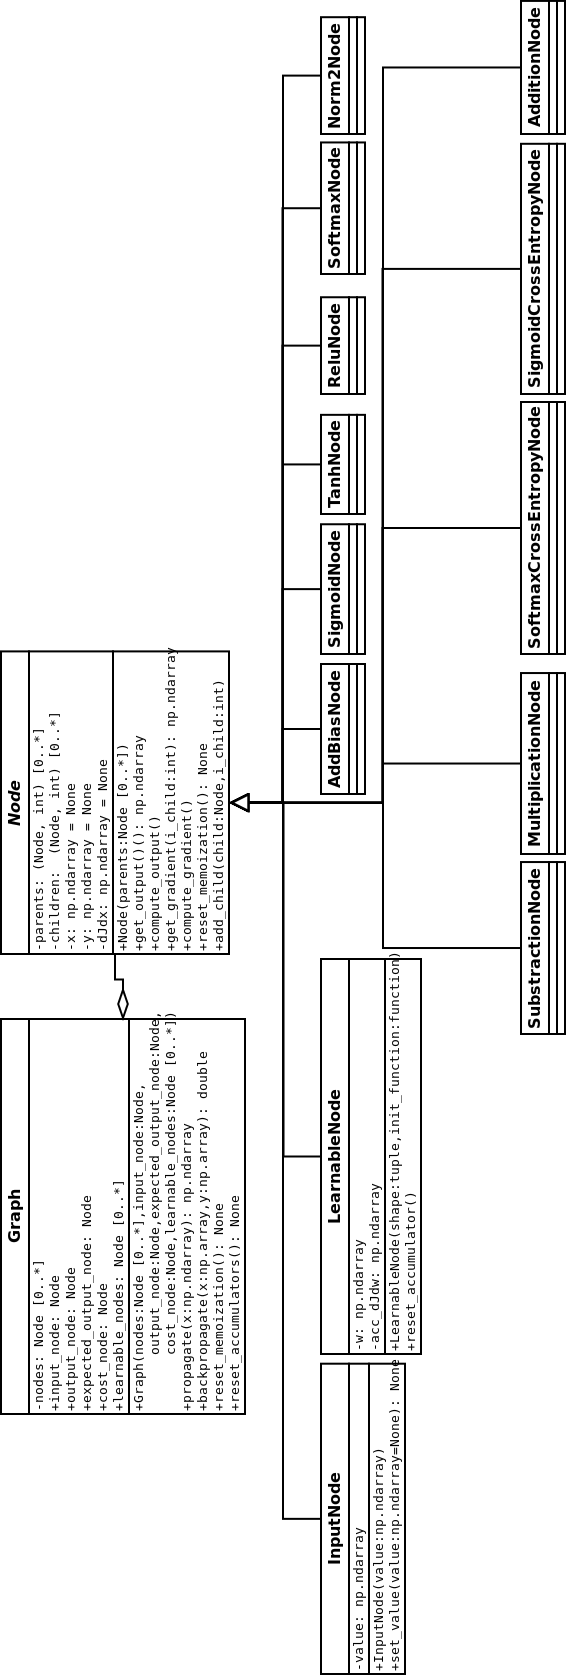
\includegraphics[scale=0.3]{images/chapter3/pychain_uml.png}
\caption{Diagramme UML de \texttt{pychain}}
\end{center}
\end{figure}

\section{Conclusion}

Nous avons décrit les graphes de calculs, donnés les algorithmes permenttant de calculer efficacement la sortie de celui-ci et de calculer la dérivée du coût par rapport aux paramètres. Ensuite, nous sommes rentrés davantage dans les détails en donnant les formules de propagation et de rétropropagation pour les n\oe{}uds les plus utiles dans le cadre de l'apprentissage automatique. Finalement nous avons décrit notre implémentation en donnant le diagramme de classes.

Dans cette partie, nous avons développé un outil bien plus puissant que les réseaux de neurones. En effet, nous avons donné un cadre et une méthode permettant d'optimiser théoriquement n'importe quelle fonction pour peu que nous puissions la décomposer en opérations dont nous sachons calculer la dérivée. Cette grande puissance théorique vient de plus avec une grande facilité d'implémentation et d'utilisation.

Nous verrons dans la partie suivante que notre implémentation graphes de calculs est bien plus performante que notre précédente modélisation en neurones. En outre, la modularité des graphes de calculs, nous permettra d'exécuter de nombreux tests sur l'architecture et les paramètres des réseaux de neurones, ce que nous détaillerons dans la partie suivante.

Finalement, comme nous le verrons, cette implémentation restera valide pour la modélisation des réseaux de neurones récurrents.